\subsection{Постановка задачи на разработку программы}
Программа должна соответствовать требованиям, представленным в 
Техническом Задании.

\bigskip
Задачи работы (серверная часть приложения):

\smallskip
\begin{my_enumerate}
  \item Реализовать REST API:
    \begin{my_enumerate}
      \item Обработка запросов для работы со списками покупок пользователей
      \item Обработка запросов для кроулера
      \item Обработка запросов для получения списка актуальных акционных
        товаров
      \item Обработка запросов для авторизации пользователей
    \end{my_enumerate}
  \item Спроектировать базу данных для хранения:
    \begin{my_enumerate}
      \item Акционных товаров
      \item Аккаунтов пользователей
      \item Списков покупок пользователей
    \end{my_enumerate}
\end{my_enumerate}

\bigskip
Задачи работы (клиентская часть приложения):

\smallskip
\subsubsection{Состав выполняемых функций. Клиентская часть.}
\begin{my_enumerate}
  \item Реализовать возможность просмотра списка доступных магазинов с акционными товарами
  \item Реализовать представление текущих акций для конкретного магазина:
    \begin{my_enumerate}
      \item В виде общего списка
      \item По категориям
    \end{my_enumerate}
  \item Реализовать возможность регистрации и авторизации пользователей в системе для
    работы со списком покупок
  \item Реализовать cоздание и удаление списка покупок
  \item Реализовать работу со списком покупок:
    \begin{my_enumerate}
      \item Добавление и удаление товаров магазинов
      \item Добавление и удаление пользовательских позиций
      \item Рекомендация товаров магазинов на основе пользовательских позиций 
    \end{my_enumerate}
\end{my_enumerate}

\subsection{Описание алгоритма и функционирования программы}

\subsubsection{Описание базы данных}
\begin{figure}[H]
    \centering
    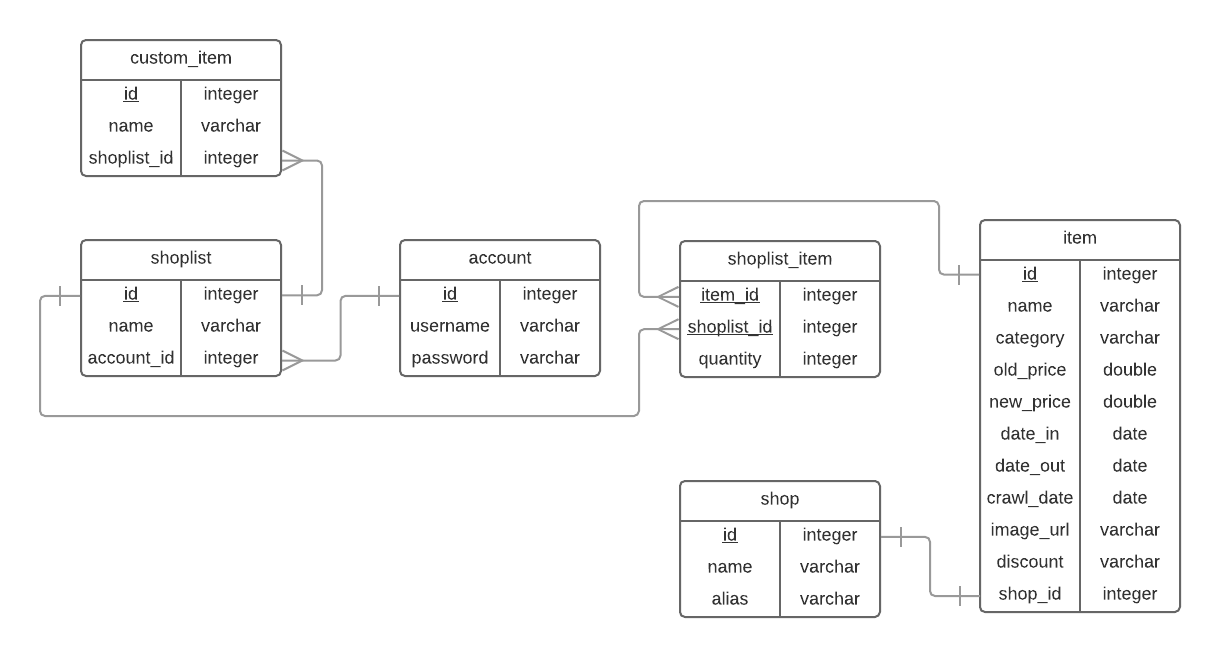
\includegraphics[width=\textwidth]{./pics/database.png}
    \caption{\small{Схема базы данных}}
    \label{database}
\end{figure}

Пожалуй, главной сущностью в схеме является "item". Именно в эту таблицу
записываются товары, собранные кроулером, и из этой таблицы извлекаются данные
для отображения в клиентских приложениях. Каждый товар также связан с
магазином, которому он принадлежит. (Один магазин может иметь много товаров).

Как видно из Рис. 1, пользователь может иметь несколько списков покупок,
которые в свою очередь могут содержать много товаров.

Серверная часть приложения написана на NodeJS и использует ORM Sequelize.
Каждая таблица в схеме базы данных имееет свое отражение в виде объекта в
программном коде. Отношения (one-to-one, one-to-many и many-to-many) задаются
через класс Association. \cite{sequelize}

\begin{minted}{javascript}
// Модель таблицы account в виде объекта в JS коде
module.exports = function(sequelize, DataTypes) {
  return sequelize.define('account', {
    id: {
      type: DataTypes.INTEGER,
      allowNull: false,
      primaryKey: true,
      autoIncrement: true
    },
    username: {
      type: DataTypes.STRING,
      allowNull: false
    },
    password: {
      type: DataTypes.STRING,
      allowNull: false
    }
  });
};

// Пример отношений между сущностями
Account.hasMany(ShopList); // Один аккаунт имеет много списков покупок
ShopList.belongsTo(Account); // Список покупок принадлежит одному аккаунту
Item.belongsToMany(ShopList, { through: ShopListItem }); // Товар принадлежит
                                            // многим спискам покупок
ShopList.belongsToMany(Item, { through: ShopListItem }); // Список покупок
                                            // принадлежит многим товарам
\end{minted}


\subsubsection{Список покупок}
Список покупок имеет следующую структуру:
\begin{my_enumerate}
  \item Имя списка покупок (Например, "Завтрак")
  \item Список товаров магазинов (Например, "Молочный коктейль Чудо детки
    шоколад; клубника 2,5\%, 200 мл")
  \item Пользовательские позиции (Например, "Сок")
  \item Итоговая сумма покупок
\end{my_enumerate}

При добавлении пользовательской позиции в список покупок, система предложит
пользователю актуальные товары из магазинов.\\
Так, например, для позиции "Сок" будут предложены следующие товары, 
которые пользователь может добавить в список товаров магазинов:
\begin{my_enumerate}
\item Сок Сады Придонья Яблоко зеленое 125мл
\item Сок Добрый Яблочный 2л
\item Десерт Джелео многослойный с соком вишня-персик-яблоко 0,4\%, 150 г
\end{my_enumerate}

Список товаров магазинов и предложенные товары на основе пользовательских
позиций для удобства группируются по магазинам.
Добавлять товары в список покупок могут только авторизованные пользователи.


\subsubsection{Описание API}
В этом разделе перечислены все endpoint'ы для реализованного API.
Для каждого endpoint'а приведено краткое описание и пример ответа в формате
json.

\textbf{Работа со списком акций}

\noindent
/api/shops -- получить список всех магазинов\\
GET-запрос\\
Пример ответа:
\begin{minted}{json}
[
    {
        "id": 1,
        "alias": "dixy",
        "name": "Дикси"
    },
    {
        "id": 2,
        "alias": "perekrestok",
        "name": "Перекресток"
    }
]
\end{minted}

\noindent
/api/shops -- загрузить новые товары на сервер. Этот endpoint нужен для
кроулера, чтобы записать собранные акции в базу данных. \\
POST-запрос\\
Тело запроса:
\begin{minted}{json}
{
    "name": "Компот Д из персиков, 580 мл",
    "category": "Консервы, соусы",
    "oldPrice": 137,
    "newPrice": 99.99,
    "dateIn": "2018-04-02",
    "dateOut": "2018-04-08",
    "crawlDate": "2018-04-02",
    "condition": "-",
    "image": null,
    "imageUrl": "https://dixy.ru/upload/iblock/fe2/2000183687.jpg",
    "discount": "-27",
}
\end{minted}

\noindent
/api/shops/:shopid -- получить список товаров для данного магазина\\
GET-запрос\\
Параметры URL:
\begin{my_enumerate}
  \item shopid -- id магазина
\end{my_enumerate}
Параметры запроса (опционально):
\begin{my_enumerate}
\item category -- название категории (по умолчанию возвращаются товары всех
  категорий)
  \item page -- номер страницы (по умолчанию 1)
\end{my_enumerate}
Пример ответа:\\
/api/shops/1?category=Кулинария,\%20заморозка,\%20мороженое\&page=1
\begin{minted}{json}
{
  "count": 192,
  "rows":
  [
      {
          "id": 565,
          "name": "Мороженое Жемчужина России эскимо миндаль-карамель, 80 г",
          "category": "Кулинария, заморозка, мороженое",
          "oldPrice": 52.9,
          "newPrice": 26.45,
          "dateIn": "2018-03-15",
          "dateOut": "2018-03-28",
          "crawlDate": "2018-03-17",
          "condition": "-",
          "image": null,
          "imageUrl": "https://dixy.ru/upload/iblock/814/2000148579.jpg",
          "discount": "1+1",
          "shopId": 1
      }
  ],
  "numPages": 1
}
\end{minted}
Здесь:\\
\begin{my_enumerate}
  \item count -- общее количество товаров для данного магазина\\
  \item numPages -- всего страниц с товарами. Расчитывается как:
    $$
    Math.ceil(count / ITEMS\_PER\_PAGE), ITEMS\_PER\_PAGE=30
    $$
  \item rows -- список с товарами\\
\end{my_enumerate}
Видно, что сервер отдает данные постранично. Т.е. вместо того, чтобы
отдать сразу все 192 товара, сервер возвращает страницы, содержащие по 30 товаров.
Поля dateIn и dateOut у объекта item нужны для того, чтобы загружать только
актуальные товары из базы. Т.е. выполняется запрос вида:
\begin{minted}{sql}
SELECT * FROM item where date_in <= currDate AND date_out >= currDate
\end{minted}

\noindent
/api/shops/:shopid/categories -- получить список категорий для данного магазина\\
GET-запрос\\
Параметры URL:
\begin{my_enumerate}
  \item shopid -- id магазина
\end{my_enumerate}
Пример ответа:
\begin{minted}{json}
["Фермерские продукты","Хлеб, сладости, снеки","Овощи, фрукты, грибы","Товары
для животных","Товары для мам и детей","Консервы, орехи, соусы","Макароны,
крупы, специи","Мясо, птица, деликатесы","Соки, воды, напитки","Молоко, сыр,
яйца","Авто, дом, сад, кухня","Наши марки","Рыба и морепродукты","Красота,
гигиена, бытовая химия","Кофе, чай, сахар","Замороженные продукты","Здоровый
выбор"]
\end{minted}

\textbf{Работа со списком покупок}

\noindent
Все запросы из этого раздела должны быть авторизваны. (см. раздел Авторизация)

\noindent
/api/shoplist -- получить списки покупок для данного пользователя\\
GET-запрос\\
Параметры запроса:
\begin{my_enumerate}
  \item mode -- режим для загрузки списков покупок
    \begin{my_enumerate}
      \item preview -- списки покупок загружаются в сжатом виде
      \item full -- списки покупок загружаются в полном виде
    \end{my_enumerate}
    Если параметр не задан, то загружаются списки покупок без товаров
\end{my_enumerate}
Примеры ответа:\\
/api/shoplist
\begin{minted}{json}
[
    {
        "id": 17,
        "name": "Купить"
    },
    {
        "id": 18,
        "name": "Чё купить"
    },
    {
        "id": 19,
        "name": "Zzz"
    }
]
\end{minted}
/api/shoplist?mode=preview
\begin{minted}{json}
[
    {
        "id": 17,
        "name": "Купить",
        "items": [
            "Мыло Солнышко хозяйственное с ароматом лимона 140г",
            "Крем-мыло жидкое Особая серия овсяное молочко, 1000 г"
        ],
        "customItems": [
            "Мыло"
        ]
    },
    {
        "id": 18,
        "name": "Чё купить",
        "items": [
            "Мешок для мусора Фрекен БОК 35л 15шт",
            "Сок Добрый Яблочный 2л",
            "Сосиски Молочные Велком, 530 г",
            "Нектар Добрый апельсиновый; мультифруктовый; персик-яблоко; груша; виноград-гранат; сок яблочный осветленный; томатный, 1 л"
        ],
        "customItems": [
            "сок",
            "колбаса"
        ]
    }
]
\end{minted}
/api/shoplist?mode=full
\begin{minted}{json}
[
    {
        "id": 17,
        "name": "Купить",
        "items": [
            {
                "id": 294,
                "name": "Мыло Солнышко хозяйственное с ароматом лимона 140г",
                "category": "Красота, гигиена, бытовая химия",
                "oldPrice": 0,
                "newPrice": 27.9,
                "dateIn": "2018-03-30",
                "dateOut": "2018-04-20",
                "crawlDate": "2018-03-30",
                "condition": null,
                "image": null,
                "imageUrl": "https://perekrestok.ru/src/product.file/list/image/21/67/16721.jpeg",
                "discount": null,
                "shop": {
                    "id": 2,
                    "alias": "perekrestok",
                    "name": "Перекресток"
                }
            },
            {
                "id": 73880,
                "name": "Крем-мыло жидкое Особая серия овсяное молочко, 1000 г",
                "category": "Непродовольственные товары",
                "oldPrice": 89.9,
                "newPrice": 44.95,
                "dateIn": "2018-04-02",
                "dateOut": "2018-04-08",
                "crawlDate": "2018-04-02",
                "condition": "-",
                "image": null,
                "imageUrl": "https://dixy.ru/upload/iblock/267/2000267119.jpg",
                "discount": "1+1",
                "shop": {
                    "id": 1,
                    "alias": "dixy",
                    "name": "Дикси"
                }
            }
        ],
        "customItems": [
            {
                "id": 24,
                "name": "Мыло",
                "shoplistId": 17,
                "matchingItems": [
                    {
                        "id": 187,
                        "name": "Крем-мыло жидкое Dove Красота и уход 250мл",
                        "category": "Красота, гигиена, бытовая химия",
                        "oldPrice": 0,
                        "newPrice": 259,
                        "dateIn": "2018-03-30",
                        "dateOut": "2018-04-20",
                        "crawlDate": "2018-03-30",
                        "condition": null,
                        "image": null,
                        "imageUrl": "https://perekrestok.ru/src/product.file/list/image/74/74/7474.jpeg",
                        "discount": null,
                        "shop": {
                            "id": 2,
                            "alias": "perekrestok",
                            "name": "Перекресток"
                        }
                    }
                  ]
            }
        ]
    }
]
\end{minted}
В этом примере видно, что помимо списка items, соответствующего товарам
магазинов, также есть список customItems, которой представляет пользовательские
позиции. У каждой пользовательской позиции есть список matchingItems, который
содержит товары магазинов, удовлетворяющих данной позиции. Также у каждого
товара есть поле shop, с помощью которого можно определить, какому магазину
принадлежит данный товар, чтобы, например, сгруппировать товары в списке покупок
по магазинам.

\subsubsection{Авторизация}
Для доступа к списку покупок пользователю необходимо авторизоваться.
Авторизация на сервере выполняется следующим образом:
\begin{my_enumerate}
  \item Пользователь авторизуется в системе, вводя свои логин и пароль
  \item Если данные верны, система возвращает токен
  \item Полученный токен клиентское приложение добавляет в заголовок
    каждого защищенного запроса
\end{my_enumerate}

Токен имеет формат JWT и представлен в следующем виде:
\begin{center}
  xxxxx.yyyyy.zzzzz
\end{center}
где\\
xxxxx -- Header (заголовок). В нем содержится метаинформация, такая как алгоритм шифрования и тип токена (как правило это JWT)\\
yyyyy -- Payload -- здесь содержится основная информация, в частности время создания токена, имя и id пользователя, получившего токен.\\
zzzzz -- Signature -- сигнатура токена. Позволяет проверить, что токен не был
подменен и является валидным. Получается в результате применения SHA256 функции:
SHA256(Header, Payload, Secret key), где Secret key -- секретный ключ, хранящийся на сервере. \\
Каждая часть токена закодирована в формат Base64.

Для авторизации в API есть два endpoint'a
\begin{my_enumerate}
  \item /auth/register -- для регистрации в системе
  \item /auth/login -- для входа в систему
\end{my_enumerate}

В обоих случаях в теле реквеста передается следующая информация: 
\begin{minted}{json}
  {
    "username": "Имя пользователя",
    "password": "Пароль"
  }
\end{minted}

В случае регистрации возвращается статус 200, если регистрация прошла успешно
или статус 500, если пользователь ввел короткое имя или пароль, либо такое
имя пользователя уже существует.

В случае успешного логина возвращается токен. Клиентские приложения должны
сохранить его, чтобы в следующий раз отправлять авторизованные запросы.
Например, в реализованном веб приложении такой токен сохраняется в локальном хранилище
(localStorage). \cite{localstorage}

\subsubsection{Клиентское веб-приложение}
Реализованное веб-приложение является SPA (Single Page Application).
Таким образом, все данные загружаются с сервера асинхронно с использованием
технологии AJAX и модификацией DOM-дерева, контент страницы изменяется
динамически.

Приложение написано с использованием JavaScript-фреймворка VueJS и включает
следующие компоненты: 
\begin{my_enumerate}
  \item App.vue -- главная компонента приложения, являющаяся родительским
    контейнером для остальных компонент.
  \item Discounts.vue -- компонента для отображения списка акций
  \item Header.vue -- компонента для навигации по сайту
  \item ItemSmall.vue -- компонента для отображения товара в списке покупок и в
    рекомендациях
  \item Item.vue --  компонента для отображения товара в списке акций
  \item Login.vue -- компонента для отображения формы входа в систему
  \item Register.vue -- компонента для отображения формы регистрации в системе
  \item ShopListCard.vue -- компонента для отображения карточки <<превью>>
    списка покупок
  \item ShopListPreview.vue -- компонента-превью для списков покупок
  \item ShopList.vue -- компонента для отображения списка покупок пользователя
  \item ShopListCustomItem.vue -- компонента для отображения пользовательской
    позиции
\end{my_enumerate}
Компоненты располагаются в приложении иерархически и могут быть вложены (nested
components). \cite{vue}

Взаимодействие между компонентами происходит через т.н. props (для передачи
данных от родительской компоненты дочерней) и через events (для передачи данных
от дочерней компоненты родительской). \cite{vue}

\begin{minted}{html}
  <!-- Объвление компоненты ShopListCard внутри ShopListPreview и
          передача ей объекта shoplist через props -->
  <shoplist-card :shoplist="shoplist"></shoplist-card>

  <!-- Объвление компоненты ItemSmall внутри ShopListCustomItem и
           обработка события, исходящего из дочерней компоненты  -->
  <item-small v-on:addItem="addItem($event)" >
  </item-small>
\end{minted}

\begin{figure}[H]
    \centering
    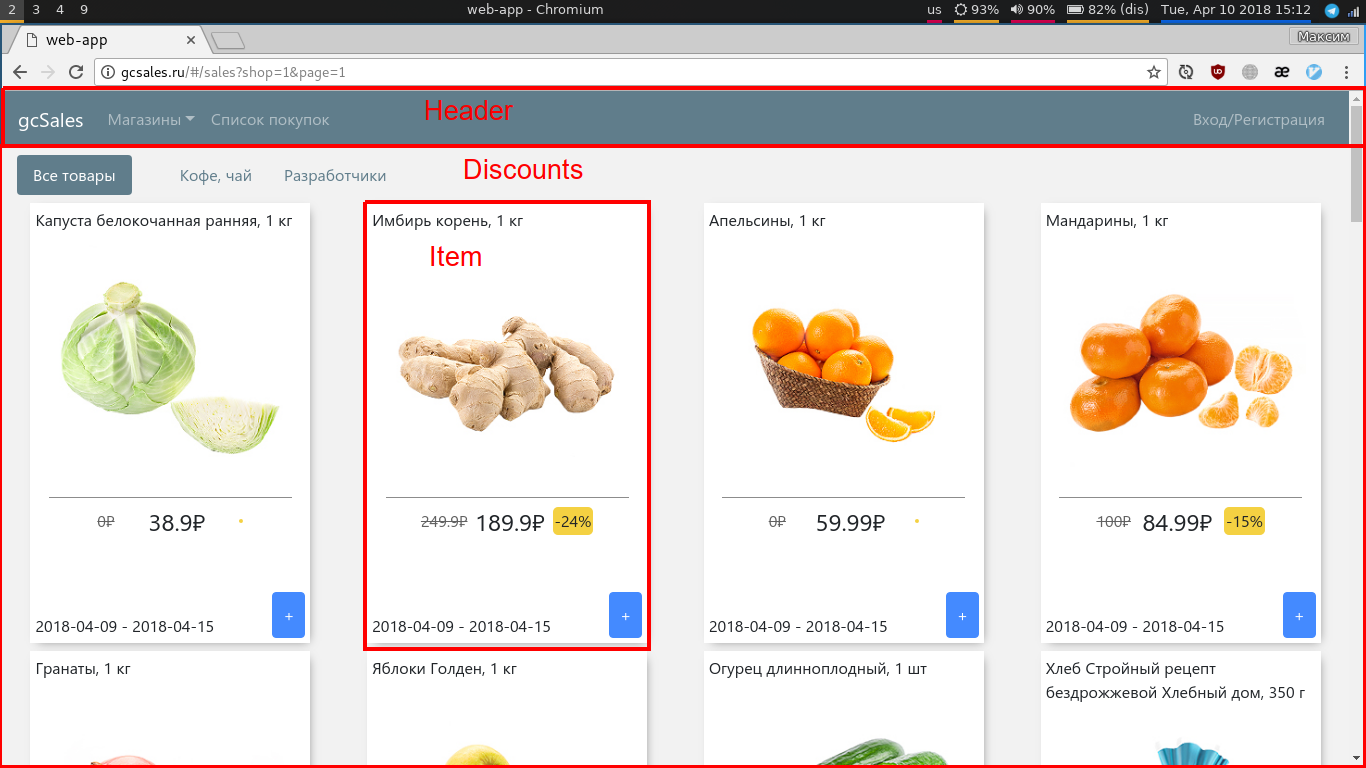
\includegraphics[width=\textwidth]{./screenshots/discounts_border.png}
    \caption{\small{Компоненты списка акций}}
    \label{database}
\end{figure}

\begin{figure}[H]
    \centering
    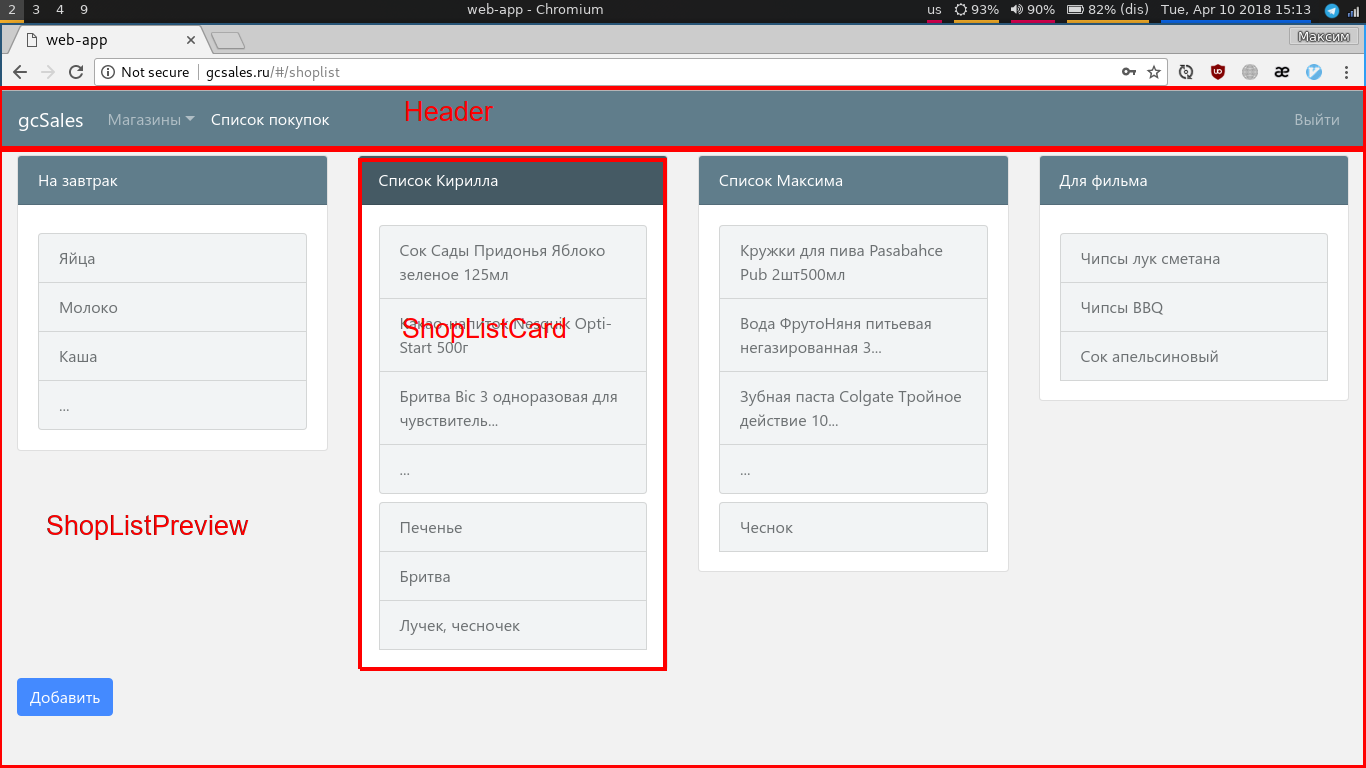
\includegraphics[width=\textwidth]{./screenshots/shoplist_preview_border.png}
    \caption{\small{Компоненты превью списков покупок}}
    \label{database}
\end{figure}

\begin{figure}[H]
    \centering
    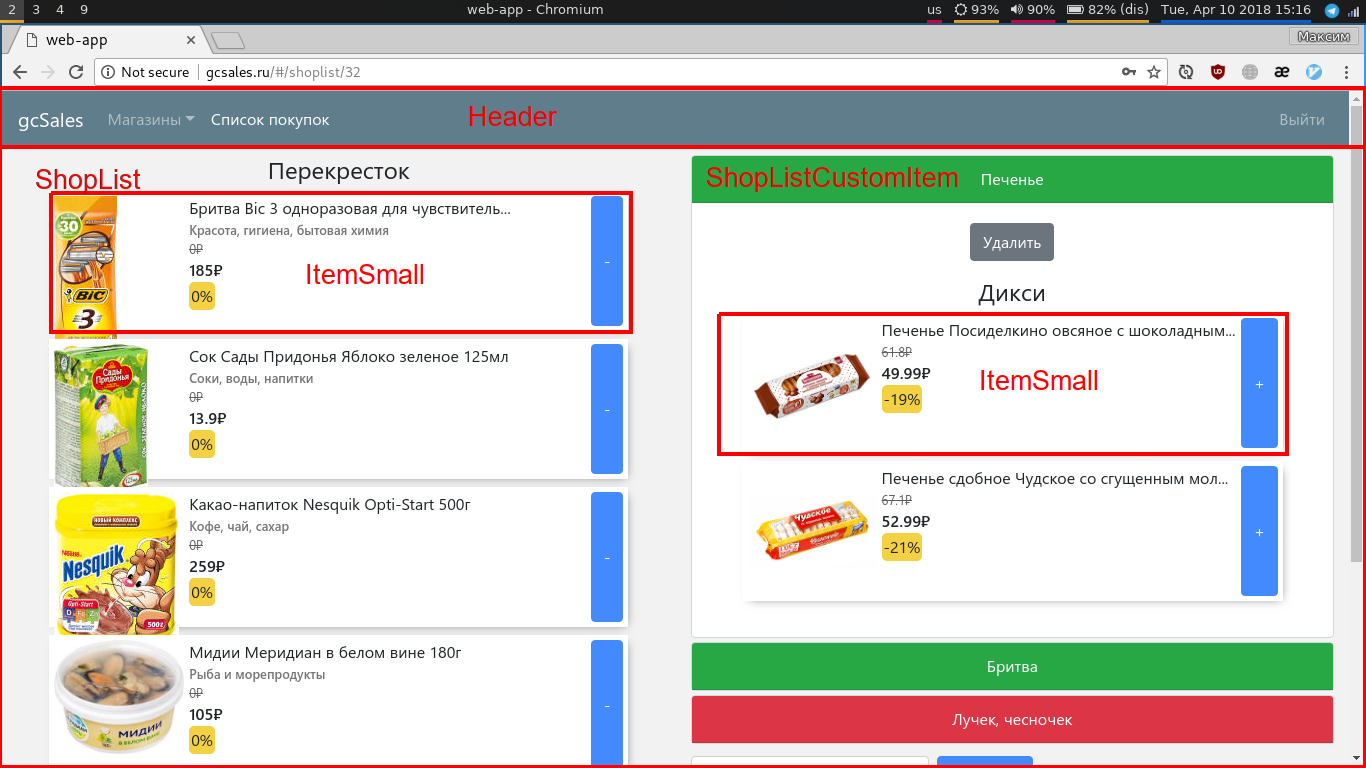
\includegraphics[width=\textwidth]{./screenshots/shoplist_border.png}
    \caption{\small{Компоненты списка покупок}}
    \label{database}
\end{figure}

\begin{figure}[H]
    \centering
    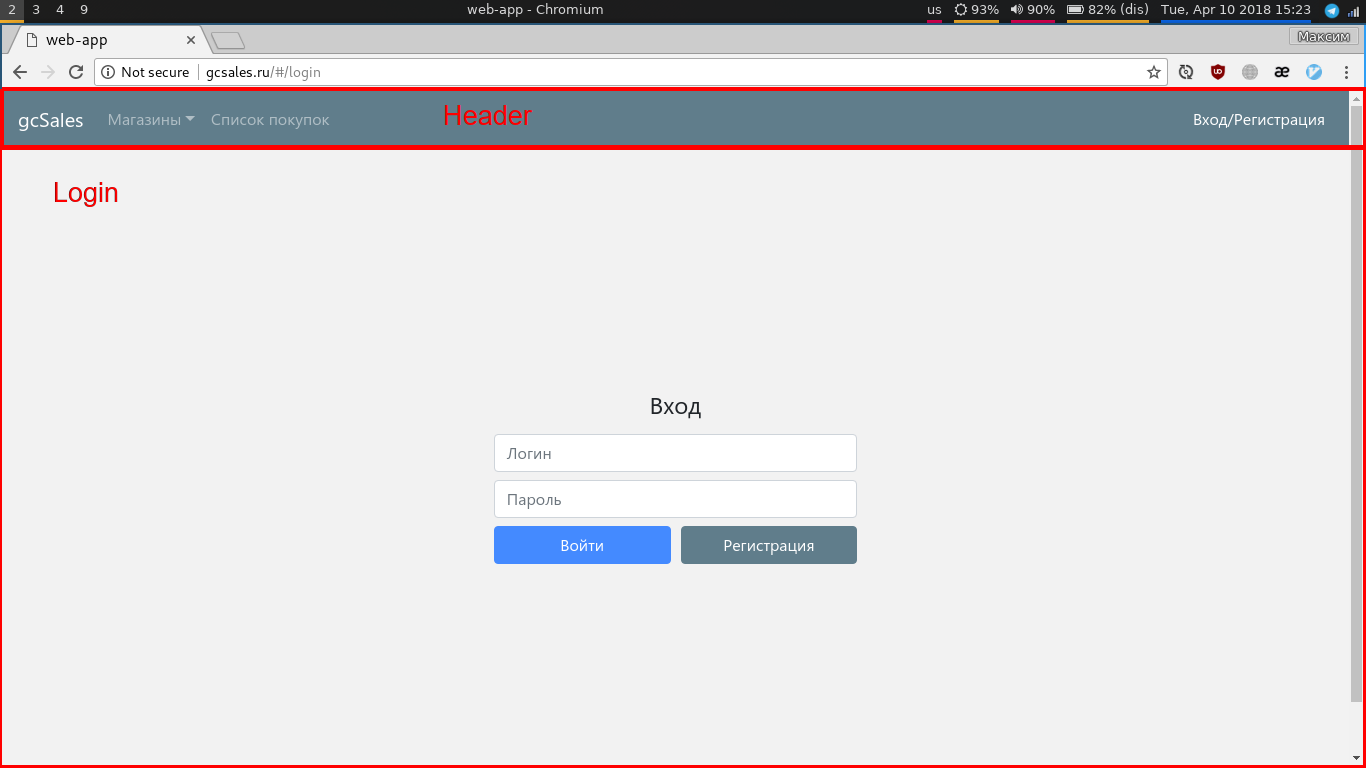
\includegraphics[width=\textwidth]{./screenshots/login_border.png}
    \caption{\small{Компоненты авторизации}}
    \label{database}
\end{figure}

\begin{figure}[H]
    \centering
    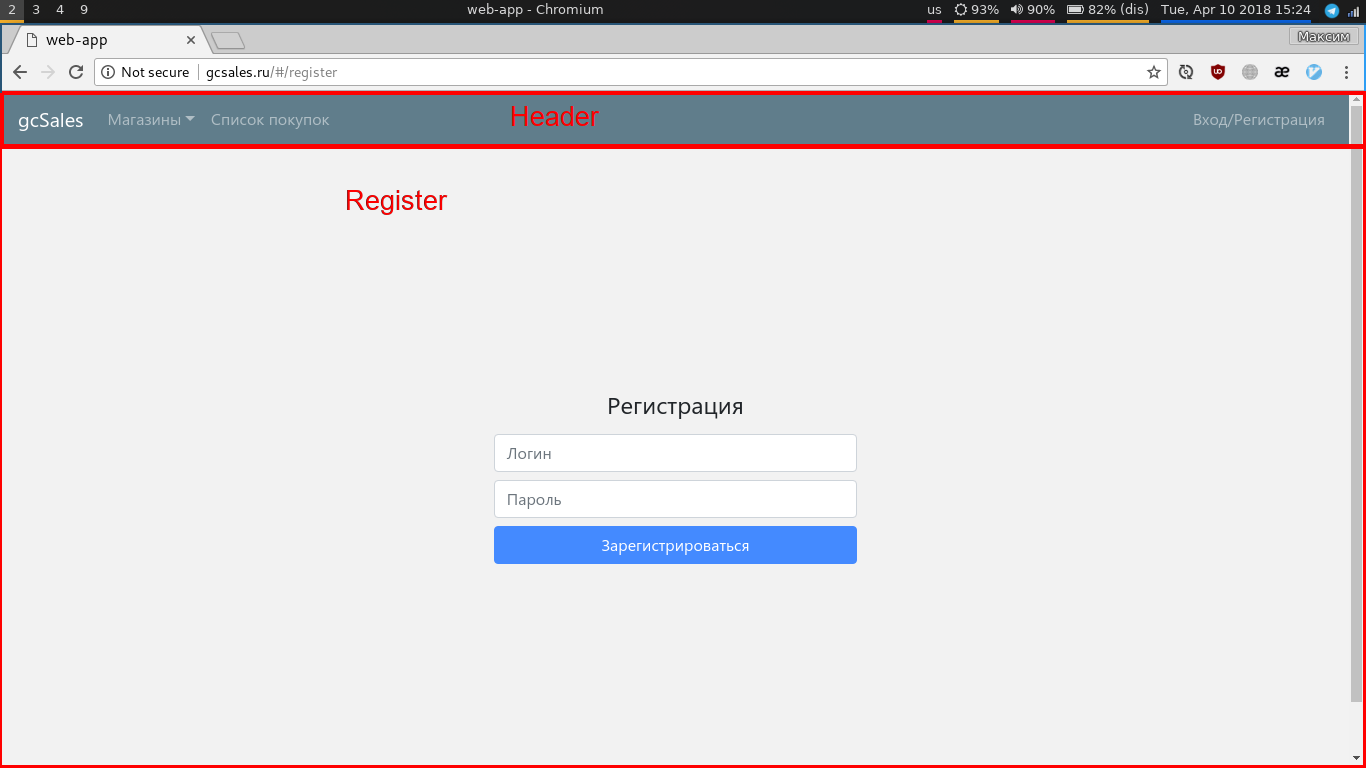
\includegraphics[width=\textwidth]{./screenshots/register_border.png}
    \caption{\small{Компоненты регистрации}}
    \label{database}
\end{figure}

\subsection{Организация входных и выходных данных}
Клиентские приложения и сервер обмениваются данными в формате JSON.

\subsection{Описание выбора состава технических и программных средств}
\subsubsection{Описание выбора состава технических средств}
Для обеспечения работоспособности программы требуются следующие
технические средства:

\begin{my_enumerate}
  \item ПК или мобильное устройство
  \item Доступ в интернет
\end{my_enumerate}

\subsubsection{Обоснование выбора состава технических средств}
Доступ в интернет необходим, т.к. веб-приложение размещено на сетевом ресурсе.

\subsubsection{Описание выбора состава программных средств}
Для запуска и работы программы требуется ПК или мобильное устройство со
следующим предустановленным программным обеспечением:

\begin{my_enumerate}
  \item Интернет-браузер Google Chrome версии 49 и выше или
  \item Интернет-бразуер Firefox версии 44 и выше
\end{my_enumerate}

\subsubsection{Обоснование выбора состава программных средств}
Выбор состава программных средств обоснован минимальными требованиями
фреймворка VueJS и библиотеки Bootstrap. \cite{caniuse}

